\documentclass[11pt,letterpaper]{article}
\usepackage{acl2013}
\usepackage{times}
\usepackage{latexsym}
\usepackage{amsmath}
\usepackage{amssymb}
\usepackage{amsthm}
\usepackage{enumerate,paralist,enumitem}
\usepackage{verbatim}
\usepackage{mathtools}

\usepackage{url}

\usepackage{array}

\usepackage{graphicx}
\usepackage{caption,subcaption}
\usepackage{algorithm}
\usepackage{algorithmic}

\DeclareMathOperator*{\argmax}{arg\,max}

%\usepackage{authordate1-4}
\usepackage{multirow}

\usepackage{color,soul}
\usepackage{transparent}
\usepackage[usenames,dvipsnames,svgnames,table]{xcolor}
\newcommand{\Note}[1]{}
\renewcommand{\Note}[1]{\hl{[#1]}}
\newcommand{\FIXME}{\Note{FIXME}}
\newcommand{\NoteSigned}[3]{{\sethlcolor{#2}\Note{#1: #3}}}
\newcommand{\RemoveFF}[1]{\NoteSigned{Remove (FF)}{Crimson}{#1}}
\newcommand{\NoteFF}[1]{\NoteSigned{FF}{LightBlue}{#1}}
\newcommand{\NoteJE}[1]{\NoteSigned{JE}{LightGreen}{#1}}

\newcommand{\empirical}[0]{\ensuremath{\tilde{p}}}
\newcommand{\Data}[0]{\ensuremath{\mathcal{D}}}

\newcommand{\WhereToFind}[0]{\url{loglin-tnlp2013.appspot.com}}
\newcommand{\NumLessons}[0]{\NoteFF{change \#: 18}}

\setlength\titlebox{6.5cm}    % Expanding the titlebox


\title{A Virtual Manipulative for Learning Log-Linear Models}


\author{
% 	 Author 1\\
% 	    XYZ Company\\
% 	    111 Anywhere Street\\
% 	    Mytown, NY 10000, USA\\
% 	    {\tt author1@xyz.org}
% 	  \And
% 	  Author 2\\
% 	    XYZ Company\\
% 	    111 Anywhere Street\\
% 	    Mytown, NY 10000, USA\\
% 	    {\tt author1@xyz.org}
 }
  
\date{}

\begin{document}

\maketitle

\begin{abstract}
We present a virtual manipulative for regularized conditional log-linear models. \WhereToFind{}
\NoteJE{also mention that our instructional materials guide the student through a series of lessons, and that we provide an accompanying handout with a more formal treatment including derivations.}
\end{abstract}

\section{Introduction}\label{sec:intro}

We argue that if one is going to teach only a single machine learning
technique in a computational linguistics course, it should be {\em
  conditional log-linear modeling}.  Such models are pervasive in
natural language processing.  They have the form
\begin{equation}\label{eqn:loglin}
p_{\vec{\theta}}(y \mid x) \propto \exp{\left(\vec{\theta} \cdot \vec{f}\left(x,y\right)\right)},
\end{equation}
where $\vec{f}$ extracts a feature vector from context $x$ and
outcome $y \in \mathcal{Y}(x)$.  The set of possible
outcomes $\mathcal{Y}(x)$ might depend on the context $x$.\footnote{In the
  case where $y$ is a binary variable, so $\mathcal{Y}(x)=\{0,1\}$,
  this model is equivalent to logistic regression.}

% Any modern course on computational linguistics or natural language
% processing needs to teach some machine learning tools.  

We then present an interactive web visualization that guides students
through playing with log-linear models and their estimation.  An
anonymized version is available for review at \WhereToFind{}.  This
open-source tool is intended to develop intuitions, so that basic
log-linear models can be then taken for granted.  It can be used near
the start of a course, perhaps after introducing probability notation
and $n$-gram models. 

The code includes \NumLessons{} ready-to-use lessons that can be used
for individual or small-group study.  Each lesson guides the student
through a manipulative exercise that centers on fitting some model
$p_{\vec{\theta}}(y \mid x)$, where ${\cal Y}(x)$ is a collection of
shapes, words, or images such as parse trees.  Each lesson is peppered
with questions, and students could be asked to answer some of these
questions in writing.\footnote{We found that answering {\em all} the
  questions\NoteJE{how many?} took them from ???--???
  words\NoteJE{Frank, fill in based on the submitted homeworks}, which
  was probably both unreasonable and unnecessary.}\NoteJE{We might
  consider releasing a couple of pencil-and-paper problems from past
  exams.}  Other instructors can add new lessons by writing 
configuration files (see section~\ref{sec:tailoring}).

\nocite{klein-tnlp-2005}\NoteFF{Is it worthwhile to cite Klein (2005)?
  In it, Klein describes the statistical NLP course he taught in 2004,
  where one of the assignments was to build a maxent POS
  tagger.}\NoteJE{Probably not: he said he was going to remove this
  assignment next time because it was too slow to train!  However, I
  think it would be helpful (maybe in the final version?) to list
  other people's NLP homework assignments or practical exercises that
  use maxent.  I bet you could find a few good assignments on the web,
  including in the NLTK book.}

\section{Why Teach With Log-Linear Models?}

Log-linear models are very handy in NLP.  They can be used {\em throughout} 
a course, whenever one needs 
\begin{itemize}
\item a global classifier for an applied task, such as detecting
  sentiment, topic, spam, or gender;
\item a local classifier for structure annotation,
  such as tags or segment boundaries;
\item a local classifier to be applied repeatedly in sequential decision-making;
\item a conditional probability within some generative process, such
  as an $n$-gram model, HMM, PCFG, probabilistic FSA or FST, noisy-channel MT model,
  or Bayes net;
\item a global structured prediction method---here $y$ is a structured
  object from a large space of possible outputs.  (Then $p(y \mid x)$ is a
  Markov random field or a conditional random field, depending on whether 
  $x$ is empty or not.)
\end{itemize}  

Log-linear models over discrete variables are also sufficiently
expressive for an NLP course.  Students can experiment freely with
adding linguistically interesting features of their own devising,
since the probability \eqref{eqn:loglin} may consider any number of
informative features of the $(x,y)$ pair.

How about training?  Estimation of the parameter weights
$\vec{\theta}$ from a set of fully observed $(x,y)$ pairs is simply a
convex optimization problem.  Maximizing the regularized maximum
likelihood
\begin{equation}\label{eqn:reg_ll}
% \argmax_{\vec{\theta}} \sum_i \log p_{\vec{\theta}}(y_i \mid x_i) - C\cdot R\left(\vec{\theta}\right)
  F\left(\vec{\theta}\right) = \sum_{i=1}^N \log{p_{\vec{\theta}}\left(y_i\ \mid\ x_i\right)} - C \cdot R\left(\vec{\theta}\right)
\end{equation}
is a simple, uniform training principle that can be used throughout
the course.  The regularizer $R(\vec{\theta})$
prevents overfitting on sparse features.
This is arguably more straightforward than the traditional NLP
smoothing methods for estimating probabilities from sparse data
\cite{chen-goodman-1996}, which require applying various {\em ad hoc}
formulas to counts, and which do not generalize well to settings where
there is not a natural sequence of backoff models.  There exist 
fast and usable tools that students can use to train their log-linear
models, including, among others, MegaM \cite{daume04cg-bfgs}, 
and NLTK \cite{bird2009natural}.\footnote{\label{fn:bigY}A caveat is that generic
  log-linear training tools will {\em iterate} over the set ${\cal
    Y}(x)$ in order to maximize
  \eqref{eqn:loglin} and to compute the constant of proportionality
  in \eqref{eqn:loglin} and the gradient of
  \eqref{eqn:reg_ll}.  This is impractical when ${\cal Y}(x)$ is large, as in
  language modeling or structured prediction.  One will do better to
  use specialized algorithms that exploit special structure in the
  feature set, or to fall back on sampling or variational
  approximation if no such structure is available.  In these settings,
  students will have to use other tools or write their own code.}
%\NoteJE{what else?  can we recommend one?}
%\NoteFF{I've only ever used my own so I wouldn't feel comfortable
%recommending any.}

Formally, log-linear models are a good gateway to a more general
understanding of undirected graphical models and the exponential
family, including globally normalized joint or conditional
distributions over trees and sequences.

One reason that log-linear models are both versatile and pedagogically
useful is that they explicitly model {\em probabilities}.  These can be 
\begin{itemize}
\item combined with other probabilities using the usual rules of probability;
\item marginalized at test time to obtain the probability that the output 
  $y$ has a particular property (e.g., one can sum over alignments);
\item marginalized at training time in the case of incomplete data $y$
  (e.g., the training data may not include alignments);
\item used to choose among possible outputs by computing their 
  expected loss (risk).
\end{itemize}
The training procedure also takes a probabilistic view.  Equation
\eqref{eqn:reg_ll} illustrates important statistical principles such as maximum
likelihood, regularization, and cross-validation, as well as
optimization principles such as gradient ascent.\footnote{In an
  advanced class, this objective can also be regarded as the
  optimization dual of a maximum entropy problem.}

For all these reasons, we recommend log-linear models as one's
``go-to'' machine learning technique when teaching.  Other linear
classifiers, such as perceptrons and SVMs, similarly choose $y$ given
$x$ based on a linear score $\vec{f} \cdot \vec{\theta}(x,y)$---but
these scores have no probabilistic interpretation, and the procedures
for training $\vec{\theta}$ are harder to understand or to justify.
Thus, they can be taught as variants later on or in another course.
Further reading includes \cite{smith-2011}.

\subsection{History and Applications}

\NoteJE{move to an appendix?}%
\NoteFF{I like this in here. We might want to comment out some initially
  but add it back in if any camera-ready allows for additional spaces}%
\NoteJE{It's just that I don't want to keep the reader from getting to
  the fresh stuff that we are presenting in the paper.  Possibly YOU found this 
  more interesting than the visualization because you were already 
  overly familiar with the visualization.  But the reader hasn't seen 
  the visualization before and is presumably impatient to get to it.
  It's true that the section is not that long, so I dunno.  But it's not that
  important either, even though it was slow to write.}

Conditional log-linear models were first popularized in computational
linguistics by a group of researchers associated with the IBM speech
and language group, who called them ``maximum entropy models,'' after
a principle that can be used to motivate their form
\cite{jaynes-1957}.  They applied the method to various binary or
multiclass classification problems in NLP, such as prepositional
phrase attachment \cite{ratnaparkhi-1994}, text categorization
\cite{nigam-lafferty-mccallum-1999}, and boundary prediction
\cite{beeferman-berger-lafferty-1999}.

Of particular importance for NLP, these models can be also used for
structured prediction problems such as tagging, parsing, chunking,
segmentation, and language modeling.  A simple strategy is to reduce
structured prediction to a sequence of multiclass log-linear
predictions \cite{ratnaparkhi-1998}.  A more global approach---used in
the original ``maximum entropy'' papers---is to use \eqref{eqn:loglin}
to define the conditional probabilities of the steps in a generative
process that gradually produces the structure
\cite{rosenfeld-1994,berger-dellapietra-dellapietra-1996}.  This idea
remains popular today and can be used to embed rich distributions
into a variety of generative models \cite{bergkirkpatrick-et-al-2010}.
For example, a PCFG that uses richly annotated nonterminals involves a
large number of context-free rules.  Rather than estimating their
probabilities separately, or with traditional backoff smoothing, a
simpler approach is to use \eqref{eqn:loglin} to model the probability
of all rules given their left-hand sides, based on features that
consider subsets of the nonterminal annotations.\footnote{E.g., case,
  number, gender, tense, aspect, mood, lexical head.  In the case of a
  terminal rule, the spelling or morphology of the terminal symbol can
  be considered.}  A final approach to structured prediction is to
simply predict the structured output all at once, so that $y$ is a
large structured object.  Since it is hard to enumerate
a large set of possible outputs ${\cal Y}(x)$ (see footnote
\ref{fn:bigY}), one can either restrict ${\cal Y}(x)$ before training
\cite{johnson-et-al-1999}, or else use techniques such as dynamic
programming or sampling, as in linear-chain conditional random fields
\cite{lafferty-mccallum-pereira-2001} and whole-sentence language
modeling \cite{rosenfeld-chen-zhu-2001}.

\section{The Teaching Challenge} \label{sec:challenges}

Unfortunately, there is a difficulty with introducing log-linear
models early in a course.  Once grasped, they seem very simple.  But
they are not so easy to grasp for a student who has not had any
experience with high-dimensional parametric functions or with
statistical estimation.  The interaction among the parameters can be
bewildering.  Log-likelihood, gradient ascent, and overfitting may also
be new ideas.

Students who lack intuitions about these models will fail to follow
subsequent lectures.  They will also have trouble with homework
projects---interpreting the weights learned by their model, and
diagnosing problems with their features or their implementation.  A
student cannot even design appropriate feature sets without
understanding how the weights of these features interact to define a
distribution.  We will discuss some of the necessary intuitions in
sections \ref{sec:aims} and \ref{sec:lessons}.

We would like equations \eqref{eqn:loglin} and \eqref{eqn:reg_ll} and the
gradient formula to be more than just recipes.  The student should
regard them as {\em familiar objects with predictable behavior}.  Like
computer science, pedagogy proceeds by layering new ideas on top of
already-familiar abstractions.  A solid understanding of basic
log-linear models is prerequisite to 
\begin{itemize}
\item using them in NLP applications that have their own complexities, 
\item using them as component distributions within larger probability
  models or decision rules,
\item generalizing the algorithms for working with \eqref{eqn:loglin}
  and \eqref{eqn:reg_ll} to settings where one cannot easily enumerate
  ${\cal Y}$.
\end{itemize}

\section{Manipulatives}

\NoteJE{Start by explaining the use of manipulatives in early math
  education, perhaps including an example and a quote.  I tried to set
  this up at the end of the previous section by talking about
  ``familiar objects with predictable behavior.''  The bottom line is
  that we'd like students to develop \emph{physical} intuitions about
  these abstract models.}

\NoteFF{what is the history of virtual manipulatives in teaching CS? NLP?} the HMM spreadsheet \cite{eisner-2002-tnlp}

%except for reading of data files, purely client-side $\Rightarrow$ very easy to set-up;
%open-source;
%data input format makes it extensible;
%individual lessons can be tailored (e.g., hide/show buttons, different tool-tips for lessons)

Why do we focus on shapes, rather than words? \NoteFF{maybe we can argue via virtual manipulatives}\NoteJE{yes}

%%%%%%%%%%%%%%%%%%%%%%%%%%%%%%%%%%%
%%%%%%%%%%%%%%%%%%%%%%%%%%%%%%%%%%%
%%%%%%%%%%%%%%%%%%%%%%%%%%%%%%%%%%%

\section{Pedagogical Aims}\label{sec:aims}

\NoteJE{This key section is a bit hard to read and especially to skim.
  It has too much repetitive padding about our desires, and what the
  students must do, and how ``important'' it is.  Instead, could we
  just list the facts about log-linear models that we want students to
  appreciate?  (You should be able to harvest these by going through
  the lessons.)  That is, it would be crisper to stay focused on the
  properties of the model rather than referring repeatedly to the
  people.  See for example the bullet points in section 3 of
  eisner-2002-tnlp, although you don't necessarily need to follow that
  format.}

We wish to make log-linear models a concept that students can reason
about quickly and intuitively. We found that expanding upon the
difficulties from Section \ref{sec:challenges} and listing specific
pedagogical goals helped focus the design of the virtual manipulative
and hone the creation and expected take-aways of individual
lessons.\NoteJE{True but boringly meta. We also used section headers
  because we found them useful to organize the paper, but we don't
  have to say so. :-) Just list the goals or better yet the facts.
  They'll speak for themselves.}

\subsection{Modeling Implications\NoteJE{I don't understand this
    (ambiguous) section title}}

Given $N$ data points $\Data{} = \{( x_i, y_i)\ \mid\ 1 \le i \le N\}$, one of the initial, and perhaps most important, decisions 
to make is choosing an appropriate model and distribution family. As argued above, for this manipulative we focus on 
contrasting exponential families \eqref{eqn:loglin} with what students may iniitally posit, the empirical distribution:
\begin{equation}
\empirical\left(y\ \mid\ x\right) = \frac{c(x,y)}{c(x)}.
\label{eqn:empirical_distr}
\end{equation}
%where $c(x,y)$ and $c(x)$ represent bigram and unigram counts, respectively.
While perhaps pragmatically the most important consequence of this modeling decision is that of 
proper feature design, we wish students to consider additional implications.  
How does \eqref{eqn:loglin} generalize other distributions: $\vec{\theta} = 0$ 
yields the uniform distribution, but can one match the empirical? What constraints does 
the model satisfy?
%How does this relate to the maximum entropy view?
% (if any; eg., maxent formulation or empirical
%MLE?)
 
We also wish to impart the differences between conditional models and
globally normalized ones
$\hat{p}_{\vec{\theta}}\left(y\right)$.\NoteJE{I'd get rid of the hat
  in $\hat{p}$.  It hasn't been defined or used above, and may be
  distracting, so you could get rid of it later as well.}  Although
these context-nescient\NoteJE{???} models allow students to focus on
understanding some of the core underlying mathematical concepts of
exponential models, such as feature interations and weight tradeoffs,
there are important differences between global and conditional models
that must be understood. For instance, in conditional models features
can be ``shared'' across conditions, which can
help %the regularizer even if likelihood is the same.
generalization to unseen context-outcome pairs and maximizing the
regularized objective.

The modeler has the onus of proper feature design: when defining $K$ 
appropriate features $f_k$, there are a number of at-times complex interactions 
to consider, so the lessons and take-aways must reflect these complexities. 
First, the student must intuit what good discriminative features are: 
when defining a globally normalized model over solid circles, striped 
circles, solid triangles and striped triangles, the first features 
one might consider are contrasting indicator functions for whether a shape
is a circle or is solid. The student should be aware that opposing (binary) features 
that completely partition the outcome space (e.g., solid vs. striped features) are redundant.

Second, the student must understand the difference between \textit{type} and 
\textit{feature} counts, and how those counts affect the feature weights. 
For example, if the “solid” feature is predicted to occur less often 
than it actually does, the student must raise its weight. But since raising one weight 
may affect (significantly) the quality of all the other weight, fitting one weight in
isolation may reduce or reverse the need to raise other weights. 

In general we must show that both the number and range of features affects the expressive 
power of the model. But this expressiveness has a cost, as too many features can lead to overfitting. 
Similarly, defining features that everything (or nothing) has can make the weights 
take extreme values (go to $\pm \infty$). Further, though $f_k$ is commonly designed to be binary, 
this is not a strict requirement, and defining non-binary feature functions, such as one that fires in 
proportion to some property of the datum (e.g., the number of sides of a shape) can affect the
proportions of feature counts.

% (and the importance of regularization)

Our manipulative must generalize the above points to conditional models. In particular, students should 
understand the effect the amount of data (per context) has on what features are appropriate to define 
(e.g., that frequent conditions are more influential). It is also important to introduce backoff features 
and smoothing, and why defining those coarser features are useful. Finally, students need to know that 
features that only fire on conditions have no effect on conditional distribution.

% defined over \Data{} , we are interested in estimating distributions 
%\begin{equation}
%\hat{p}_{\vec{\theta}}\left(y\ \mid\ x\right) = \frac{u(x, y)}{\sum_{y'} u(x,y')},
%\label{eqn:conditional_loglin}
%\end{equation}
%from the unnormalized scores $u(x,y)$
%\begin{eqnarray}
%u(x,y) & = & \exp{\left(\vec{\theta}\cdot \vec{f}(x,y)\right)}.%\\
%%& = & \exp{\left(\sum_{k=1}^K \theta_k f_k(x,y)\right)}.
%\end{eqnarray}

%Therefore, we also 

\subsection{Importance of the Objective and Parameter Estimation} % and Evaluating the Model}

We summarize the model's quality via the regularized conditional
log-likelihood \eqref{eqn:reg_ll}.  $C \ge 0$ is the penalty for the
regularizer $R(\vec{\theta})$.
%The model is fully described by the feature weights $\vec{\theta}$, but weights can be fit too
%strongly to particular observations. 

The maximizer is the $\vec{\theta^*}$ that solves equation \eqref{eqn:grad}:
\begin{equation}
\begin{aligned}
%\begin{split}
\nabla_{\vec{\theta}} F
 = &
\ \mathbb{E}_{\empirical{}}\left[\vec{f}(X,Y)\right] 
- \mathbb{E}_{{\hat{p}_{\vec{\theta}}}}\left[\vec{f}(X,Y)\right]\\
 & - C \nabla_{\vec{\theta}}R(\vec{\theta})
\label{eqn:grad} \\
%= &\ \mathcal{C}(\empirical{}, p_{\vec{\theta}}) - C \nabla_{\vec{\theta}} R(\vec{\theta})\\
 = &\ 0.
%\end{split}
\end{aligned}
\end{equation}
Many important concepts are introduced in these two equations. Some are new to the student, in that he or
she was not exposed to them when considering feature design); others provide an alternative view
on concepts already introduced. It is important to highlight these connections.

We believe the most important concept is that of the non-regularized gradient being the difference between the observed
feature counts and the expected feature counts:
\begin{equation}
\ \mathbb{E}_{\empirical{}}\left[\vec{f}(X,Y)\right] 
- \mathbb{E}_{{\hat{p}_{\vec{\theta}}}}\left[\vec{f}(X,Y)\right].
\label{eqn:obsexp} 
\end{equation}
Students should already have been introduced to this when considering the difference between type and 
feature counts, and how expectation proportions affect how much one needs to change a given feature weight: 
now, with the gradient, they can better understand why, and thus justify and strengthen their developing intuitions.

While a number of students may have prior experience with numerical optimization, for those that haven't, the next 
important ideas are that ``following'' \eqref{eqn:grad} will
\begin{inparaenum}[i)]
\item actually yield a solution, even though a closed-form solution is not generally available, and
\item not decrease the objective.
\end{inparaenum}
The importance of the convexity of \eqref{eqn:reg_ll} should be introduced here as a way to generalize the 
previous two observations, notably that we will always find a unique $\vec{\theta^*}$ that solves \eqref{eqn:reg_ll}.
\footnote{Advanced students may find it interesting to see what happens when you ``break'' convexity, e.g., what 
happens when $C < 0$?}
Students should understand that matching the empirical distribution will generally maximize the (unregularized) log-likelihood, 
though that overfitting is possible and may result in a larger log-likelihood than the true generating distribution yields.
%Here, Regardless of what regularization is applied, we will generally refer to the \textbf{full model} as that of \eqref{eqn:conditional_loglin} with objective \eqref{eqn:reg_ll}.\footnote{We consider models where $R(\vec{\theta}) = \vec{0}$ (no regularization), $R(\vec{\theta}) = \|\vec\theta\|_1$, and $R(\vec{\theta}) = \|\vec{\theta}\|_2^2$. See Section \ref{sec:overview} for more on regularization.}

We may use the gradient to further illustrate feature modeling considerations. The most obvious is to show how 
minimizing a single isolated $|\frac{\partial}{\partial \theta_k} F|$ might adversely affect another partial 
$\frac{\partial}{\partial \theta_{k'}}F$, but one should also make the additional connections to type vs. feature counts 
and that even if distributions do not full match, expected counts should.

The student should take away additional general machine learning knowledge here, including how a small training set can
affect the overall estimator $\vec{\theta^*}$ (higher variance), but that regularization, which should the student should consider
to be a form of smoothing, reduces the variance at the expense of the \textit{training} log-likelihood. Thus regularization 
(smoothing) fits the data imperfectly, either because the model has fewer parameters than outcomes, or because using too 
many parameters would be penalized by the regularizer (this should be connected back to the expressiveness considerations 
introduced in feature modeling). Further, to limit regularization penalty, the model can make use of backoff features and 
not just fine-grained features, thereby resulting in backoff smoothing.

We should note that we are \textit{not} concerned with computational issues here, e.g., that of tractably computing the normalization factors $Z(x_i)$. While efficiently computing the normalization factor is a crucial component to practical log-linear models, our primary concern is to provide a virtual manipulative that imparts a near-physical, intuitive understanding of log-linear models. 

%%%%%%%%%%%%%%%%%%%%%%%%%%%%%%%%%%%
%%%%%%%%%%%%%%%%%%%%%%%%%%%%%%%%%%%
%%%%%%%%%%%%%%%%%%%%%%%%%%%%%%%%%%%

\section{Virtual Manipulative}\label{sec:overview}
\begin{figure*}
\centering
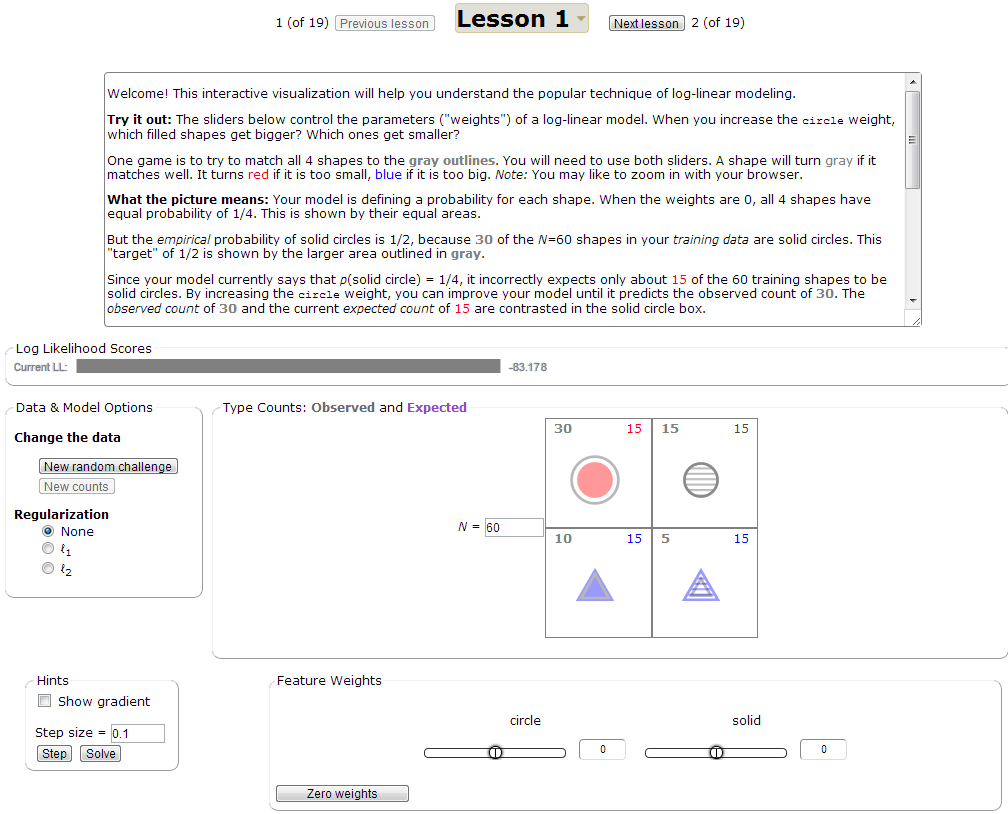
\includegraphics[scale=.5]{images/lesson1-050913-intro.PNG}
\caption{\NoteFF{Add references} Screenshot of the first lesson from the virtual manipulative.}
\label{fig:lesson1}
\end{figure*}

\NoteJE{maybe move this section before ``pedagogical aims'' so that
  the reader can find out sooner about our actual contribution,
  a.k.a. The Cool Stuff?  Then the pedagogical aims would lead right
  into the lessons or could even be combined with them.}

We have made an anonymized version available at \WhereToFind{}. 
We encourage the reader to play with it in tandem to reading this paper.

While our primary goal was to teach log-linear models within the context of NLP, 
we thought it myopic to outright limit users to those interested or experienced 
in NLP. %, due in part to the prevalence and success log-linear models boast 
%throughout a number of varied computational fields. 
\NoteJE{The next two sentences seem unnecessary since they'll be
  obvious by the end of the paper if they aren't already.  Again,
  shouldn't we spend as much time as we can on what it's like for the
  student and teacher to use the manipulative, rather than on our
  (mostly) boring and irrelevant experience of designing and coding
  it?  The goal of the paper is to sell other teachers on using the
  app.}  One of the guiding design goals was to make the educational
tool easy to use by both students and instructors, so that instructors
could tailor the lessons to the needs, interests and abilities of the
students. To that end, our manipulative has three primary components:
the student interface (front-end), important aspects transparent to
the instuctor, and the back-end implementation.

\subsection{Student Interface}
The basic unit of completion in our manipulative is a \textit{lesson},
where the aim is to further examine some subset of the goals from
Section \ref{sec:aims}.\NoteJE{Again, beware of nerdview.  How about:
  ``Each lesson addresses some of the points above.''  Even that could
  be cut, because duh.}  No matter the complexity of a lesson, the main
premise behind each is for the student to play either a ``matching
game'' or a ``log-likelihood game'' on a provided dataset \Data{}. The
data, grouped by context and presented visually at the type-level as
different shapes, images, or raw text, are modeled by two
distributions of interest: the empirical $\tilde{p}$
\eqref{eqn:empirical_distr}, and an appropriately defined log-linear
model $\hat{p}_{\vec{\theta}}$ \eqref{eqn:conditional_loglin}.  The
student controls $\hat{p}_{\vec{\theta}}$ via a slider bar, thereby
``physically'' manipulating the parameters $\vec{\theta}$.\NoteJE{And
  that makes the shapes GROW and SHRINK!  COOOOL!!!}

See Figure \ref{fig:lesson1} for the general interface.\NoteJE{I'd
  lead with this.  In fact, I think the text shown in Fig. 1 is
  extremely helpful for the reader to understand what this
  manipulative is all about, which is so far rather obscure even
  though we're well into the paper by now.  Maybe encourage the reader
  explicitly to read Fig. 1, and maybe enlarge it a bit (although the
  reader can zoom in if they're reading onscreen).  In the final
  version, you might be able to get a higher-res screenshot by zooming
  the browser (and using an appropriately large window); this gives a
  larger image and larger-font text, which you can shrink back again
  in the PDF.}  Note in particular the data area \NoteFF{ref}, the
feature weight sliders \NoteFF{ref}, and the log-likelihood score
\NoteFF{ref}. Each datum has two shapes associated with it, an
``uninteresting'' gray outline ($\empirical{}$) and a salient
``interesting'' object ($\hat{p}_{\vec{\theta}}$). The size (area) of
each shape is proportional to its probability mass, while its color
indicates whether the observed or expected count is larger.  The
number above and to the left of each datum is that type's empirical
count, while the number above and to the right is its expected count.
For instance, in Figure \ref{fig:lesson1}, the data --- 30 solid
circles, 15 striped circles, 10 solid triangles, and 5 striped
triangles --- are modeled by the two indicator features
$f_{\textrm{circle}}$ and $f_{\textrm{solid}}$. With $\vec{\theta} =
0$ we have the uniform distribution, so the solid circle is contained
in its gray outline ($\empirical{}(\textrm{solid circle}) >
\hat{p}_{\vec{\theta}}(\textrm{solid circle})$), the striped triangle
contains its gray outline ($\empirical{}(\textrm{striped triangle}) <
\hat{p}_{\vec{\theta}}(\textrm{striped triangle})$), and the striped
circle and gray outline are coincident ($\empirical{}(\textrm{striped
  circle}) = \hat{p}_{\vec{\theta}}(\textrm{striped circle})$).
\footnote{This example describes a globally normalized model, and as
  such there is only one context. See \S\ref{sec:conditionallessons}
  for conditional models.}  See Figure \ref{fig:colorsize_inventory}
for a summary of how we use size and color to indicate salient
information.

In the \textit{matching game}, the student tries to match $\hat{p}_{\vec{\theta}}$ to 
$\tilde{p}$ --- find $\vec{\theta}$ such that $\hat{p}_{\vec{\theta}}(y\mid x) 
= \tilde{p}(y\mid x)$, for all $(x,y)$. The game is to try to make all of the salient log-linear objects 
equal in size (and color) to their corresponding gray outline. The student ``wins'' once the maximum
number of log-linear objects turn gray, thereby indicating the best possible fit.
%Rather than force students to numerically compare the
%two distributions, we scale the shape's size to indicate its type's probability
%under either distribution. We represent $\tilde{p}$ by a gray 
%outline, and use colors and shading to make $\hat{p}_{\vec{\theta}}$ salient. 

An alternative game to play is the \textit{log-likelihood game}, where the goal is to
maximize the (regularized) training log-likelihood. We represent the model's objective as a scalable 
bar graph (\NoteFF{ref}), shown directly above the data, thereby providing a quick way to distill 
the overall quality of the model. The game is to make the bar as long as possible.
%As shown in \NoteFF{fix} Figure \ref{fig:llbar}, we also represent the regularization penalty
%, and the objective under the ``true'' (generating) model parameters, when known.

Note that these games are not disjoint, nor are they the only ones that can be played.
For instance, when playing the log-likelihod game, the students can think about how well 
the shapes match, particularly when more advanced concepts such as regularization and conjoined features are 
introduced. Also, the student can play a variant of the matching game, where the goal
is to match the observed and expected feature counts. The particular game being played
in each lesson is described in the instruction area (\NoteFF{ref}), which the student should
read carefully, since this may explain what the data and particular task are, justify 
modeling choices, and ask lesson-specific questions. 

%How we indicate salience is important. As already mentioned, we 
%As documented in Figure \ref{fig:colorsize_inventory}, we utilize both size and color to 
%convey these distribution changes: the three colors red, gray and blue illustrate the 
%difference between observed and expected counts, while the size (area) of the shapes 
%indicates the type's mass differences.

%What the student interfaces with must reliably allow us to achieve the goals
%laid out in Section \ref{sec:aims}. Figure \ref{fig:lesson1} illustrates the basic 
%blocked interface a user encounters. The two block areas at the top of the 
%page serve basic navigation and instructional needs while the bottom five provide 
%the requiste interactions with the model. \NoteFF{add refs to Fig {\ref{fig:lesson1}} 
%overlay.} 
%The student should read carefully the instructions, dragging the instruction 
%area larger if necessary, since this is where the instructor may explain 

\begin{figure}[t]
\centering
\small
\begin{tabular}{
>{\centering\arraybackslash}m{.18\columnwidth} 
>{\centering\arraybackslash}m{.18\columnwidth}
>{\centering\arraybackslash}m{.18\columnwidth}
>{\centering\arraybackslash}m{.18\columnwidth}}

\textbf{Quantity of Interest} & $\mathbf{<0}$ 
& $\mathbf{= 0}$ & $\mathbf{> 0}$\\ \\

$ \mathbb{E}_{\empirical{}}\left[\vec{f}\right] 
- \mathbb{E}_{{\hat{p}_{\vec{\theta}}}}\left[\vec{f}\right]$, and 
$\nabla_{\vec{\theta}} F$
& {\bf \color{red} \texttransparent{.5}{ red } }
& {\bf \color{gray}\texttransparent{.55}{ gray } }
& {\bf \color{blue} \texttransparent{.55}{ blue } }\\  \\
\vspace{.5em}
%
%$\nabla_{\vec{\theta}} F$ visualization
%& 
\includegraphics[scale=.25]{images/goldilocks-gradient-small.PNG}
%& 
\includegraphics[scale=.25]{images/goldilocks-gradient-justright.PNG}
%& 
\includegraphics[scale=.25]{images/goldilocks-gradient-large.PNG}\\ \\ 


%& $<0$ & $= 0$ & $> 0$\\\hline\hline \\
$\empirical{} - \hat{p}_{\vec{\theta}} $& 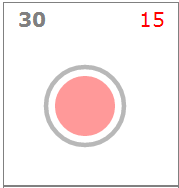
\includegraphics[scale=.25]{images/goldilocks-circle-small.PNG}
& 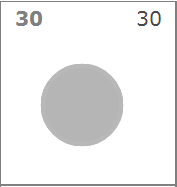
\includegraphics[scale=.25]{images/goldilocks-circle-justright.PNG}
& 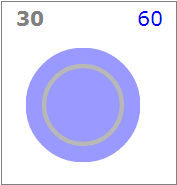
\includegraphics[scale=.25]{images/goldilocks-circle-large.PNG}\\
\end{tabular}

\caption{Colors indicate the sign of \eqref{eqn:obsexp} while the size (area) of 
the shapes indicates the difference betwen that type's probability under the 
current model and the empirical distribution (gray outline).}
\label{fig:colorsize_inventory}
\end{figure}

However, solving more complex models may be too tedious or difficult. 
The student may then make use of \textit{hints} \NoteFF{ref}, such as
viewing each component of the gradient, changing all feature weights by 
linearly following the gradient (as given by ``Step size''), or simply having
the manipulative solve the problem and providing feedback at each iteration 
of gradient ascent.

Once the student is comfortable with the provided model and data, the student
can begin to play around with the dataset and model options. These utilities, such as
generating a new random challenge and experimenting with regularizaiton, 
are described more in Section \ref{sec:lessons}.


\subsection{The Instructor Interface: Creating and Tailoring Lessons}\label{sec:tailoring}
To support a wide-range of lessons, the manipulative has support for twelve predefined shape and fill combinations.
As seen in Figure \ref{fig:shape_inventory}, the available shapes are circles, triangles, squares and pentagons,
where each can be solid, striped or hollow.

However, it is important for the instructor to be able to tailor lessons to his or her students' needs, 
interests, and abilities. For instance, it may be appropriate to reason about different types of shapes
when introducing students to log-linear models, but eventually NLP students will want to think about 
how log-linear models can be applied to NLP problems, whereas vision students will want to think about 
how to apply them to vision problems. Therefore, we have designed the manipulative to handle text
and arbitrary images as well (c.f. Figure \ref{fig:imgtxt_inventory}).

\begin{figure}[t]
\begin{center}
\begin{subfigure}[b]{\columnwidth}
\centering
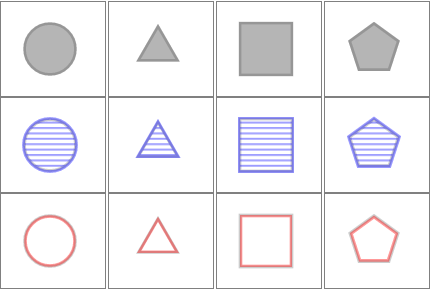
\includegraphics[scale=.5]{images/different_shapes_fills3x4.PNG}
\caption{Inventory of available shapes and fills. Note that while normally the color is indicative of the sign of \eqref{eqn:obsexp}, here the colors are solely provided as example.}
\label{fig:shape_inventory}
\end{subfigure}

\vspace{1em}
\begin{subfigure}[b]{\columnwidth}
\centering
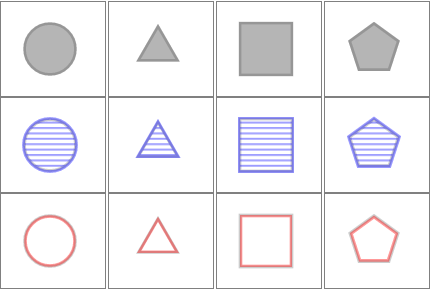
\includegraphics[scale=.5]{images/different_shapes_fills3x4.PNG}
\caption{\NoteFF{Replace with actual example text and images} Examples of including arbitrary images and text.}
\label{fig:imgtxt_inventory}
\end{subfigure}
\caption{Inventory of available shapes and objects.}
\label{fig:inventory}
\end{center}
\end{figure}

Tailoring lessons to the students' needs is as simple as editting a couple text files. These must detail:
\begin{inparaenum}[(1)]
\item a set of features, 
\item a set of contexts, and
\item for each context, a set of uniquely featurized events, including counts and visual positions.
\end{inparaenum}
These simple requirements allow one to describe some rather involved models. For example, some of 
the features may be marked as ``hidden'' to the student, thereby allowing the student to experience 
model mismatch. If the set of contexts is missing, the model is assumed to contain only 
one context and be globally normalized. Note that the visual positioning information is pedagogically 
important: aligning objects by orthogonal descriptions, e.g., circles vs. triangles or solid vs. striped, 
can make feature contrasts stand out more.

Finally, because an instructor may not want all functionality to always be available (e.g., hiding the ``solve''
capability in early lessons), we allow the instructor to declaratively make certain lesson-specific changes to 
the interface, \textit{without} going into the back-end code. 

\subsection{Back-End Implementation}
Broadly, the virtual manipulative is designed to be widely available and have minimal-to-no start-up cost. 
Aside from reading the lesson data and instruction files from the web server, the manipulative is fully 
client-side. The back-end is written in Javascript, and uses common and well-supported open-source 
libraries to help with visualization and cross-browser compatibility.\footnote{Specifically and in order, 
\texttt{d3} (\url{d3js.org/}),
\texttt{jQuery} (\url{jquery.com/}), 
\texttt{jQuery UI} (\url{jqueryui.com}),
\texttt{jQuery Tools} (\url{jquerytools.org/}), and
\texttt{qTip} (\url{craigsworks.com/projects/qtip/}).}

That being said, eventually the buck must stop somewhere and the manipulative does rely on certain HTML5 
capabilities. Unfortunately, not all current browsers support these capabilities. The manipulative works 
with recent verisons of Firefox, Chrome and Safari. We do not believe this restriction to be unreasonable, 
especially as all browers adopt widely used standards.

%The manipulative attempts to be responsive to an individual user's browser and display options, and 
%heuristically make efficient use of available space. That being said, higher resolution/larger displays 
%are desirable when dealing with the full model and some of the larger datasets introduced in later 
%lessons (see Section \ref{sec:conditionallessons}).
%
%mention that some ui considerations can result in very slight rounding errors
%
%solver: gradient ascent is simple (except for $\ell_1$ regularization), but it can take some finessing to make it visually appealing. We recursively call the solve function on a polynomial-decreasing schedule
%
%sigmoidal scaling for sliders, log-likelihood bars

\section{Provided Lessons}\label{sec:lessons}

\NoteJE{this will have to be shortened.  I suggest a narrative
  description, and encourage the reader to go try it out!}

%For instance, the student can 
%pick some new secret weights, generate a new training dataset,
%and re-estimate the weights given the new data ("New random 
%challenge"). Or 

%\item[``New Counts'' button] The other use is to help the user experiment with datasets of different sizes, by changing N to scale the counts and then clicking "New counts."
%\item[``Peek at true'']
%Regularization: We consider models where $R(\vec{\theta}) = \vec{0}$ (no regularization), $R(\vec{\theta}) = \|\vec\theta\|_1$, and $R(\vec{\theta}) = \|\vec{\theta}\|_2^2$: we special-case the optimizer to handle the non-differentiable $\ell_1$ regularization, thus providing a friendly educational environment in which the student may explore the differences between $\ell_1$ and $\ell_2$ regularization.


\subsection{Joint Models} \label{sec:jointlessons}
\begin{figure}[t]
\centering
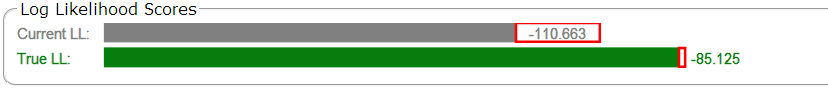
\includegraphics[scale=.3]{images/regularized_ll_bar_andtrue_cut.PNG}

\caption{The gray and green bars and text represent the (regularized) objective
 \eqref{eqn:reg_ll} for the current and empirical model, respectively. The red 
outline indicates the regularizer penalty.}
\label{fig:llbar}
\end{figure}

\begin{enumerate}
\item 
 Lead students through navigation, introduce them to helpful tooltips, ask simple understanding questions. If you make striped \& circle really big, what happens to the four probabilities?  What are the probabilities and expected counts (given N) when all features are 0?  If the total score of one object is 1 or 2 more than the total score of another object, what happens to their relative probabilities? Now try to match the gray outlines, which represent the counts you’re trying to match.  If circles overall have too low a count, you should increase circle slider: the tooltip on the slider adds up the expected and observed counts for you.  Show them the “new random challenge button.”  
\item same as lesson 1 but sliders for triangle, circle, solid, striped
Questions: What’s the difference between increasing triangle and decreasing circle?  What if you increase triangle and circle by the same amount?  Does it help at all to have 4 sliders, or could you do just as well with 2 of them? Which 2?
\item same as lesson 2 but unmatchable (“XOR problem”)
Questions: Why can’t you match the probabilities of the 4 events? But can you still use your four sliders to match the aggregate expected counts of the two features?  Is it enough to use just two of the sliders and leave the others at 0?  What kind of inductive bias does the model have -- i.e., how are the the probabilities being smoothed when you match those counts?    
Log-likelihood game. Try to predict the data "as well as you can." Slide the sliders and watch the horizontal gray bar, which gives the log-likelihood—an overall measure of how well your model predicts the training data. How long can you you make the bar? How well do the shapes then match?

Matching game. Even if you can't match all 4 probabilities with your sliders, maybe you can match the 4 features. That is, try to make your model predict that among 60 shape tokens, there would be
\item same as lesson 3, but add a single conjoined feature so it’s matchable again Questions: Does it matter which conjoined feature is added?  Would it be ok to get rid of triangle and solid as in lesson 1?
\item {triangle, square, pentagon} x {solid, striped}
a non-binary feature for number of sides: fires 3 times on triangle, 4 on square, 5 on pentagon.  Increasing this feature’s weight blows up pentagon at expense of triangle and perhaps expense of square.  Also have features for solid and for striped.
Question: what happens if you make the feature weight negative?  What would be different if if the feature were redefined from \# of sides to \# of sides - 3, or \# sides - 4?  If you added a pentagon feature, what would that allow you to do?
If this feature's weight is set to 1 (or -1), then what is the ratio of probabilities among the solid triangle, solid square, and solid pentagon? Try it! How does your answer change as you vary the weight of the solid feature?

\item %lesson 6 
rows {triangle, circle, square} X columns {solid, striped, hollow}
Questions: Is it hard to match by hand?  Learn about gradient display.
Log-likelihood game and partial derivatives; Matching game, observed circles - expected circles

Extra fun. If you enjoy trying to match the gray outlines, you can get more puzzles of this kind. Clicking "New random challenge" (at the top of the page) picks a new log-linear distribution and samples N observed events from it. Your job as a statistician is to use those N events (the gray counts and gray outlines) as clues to help you guess the true distribution. You can do a good job by playing the games above to maximize log-likelihood. Then click "Peek!" to reveal the true parameters and how well they would do on log-likelihood. (But remember lesson 2, and don't be disappointed if you found different parameters that define exactly the same distribution.)

%Warning: Reducing N before you generate the new challenge will give you fewer clues—making your statistical task harder! Your random sample of N events will be sparse and perhaps idiosyncratic. In fact, you can see the variance among random samples by clicking "New counts" to see another sample you could have gotten—with different observed counts indicated by the different-sized gray outlines. So if you try too hard to match them, you might be overfitting the training data (achieving an even better training log-likelihood than the true parameters would) rather than finding the true parameters. More about that soon ...
\item %lesson 7
Like lesson 6, but now unmatchable 
Question: Learn about solver and gradient ascent. Introduced to step size box, step button and solve button.  What solution does the model find?
``However, there will still be red and blue left on some of the shapes. How well do the expected counts for individual kinds of circles match the training data? Why?'' (actually, answer for triangles: expected = observed = 195)
\item %lesson 8
Like lesson 7, and now the solver overfits because all of the squares have count 0: so the weight goes to -infinity and we estimate the probabilities of the squares as 0, which is not good for a smoothing method.  Learn about regularization.  Question: What effect does regularization have on the expected counts of the stripes?  How about the expected counts of the others?  On the log-likelihood? why? How is this related to smoothing?  
students are encouraged to retry previous lessons to ease into regularizaiton on simpler models; \NoteFF{maybe add a screenshot of LL bar?}
\item %lesson 9 
Like lesson 7, but this time get overfitting by reducing N.  Here the student should generate a number of random challenges with different values of N, and use the solver.  Question: For a given amount of regularization, is there more smoothing of the probabilities with high N or with low N?  (Distinguish between the counts and the probabilities here.)  For a given N, is there more smoothing with high or low $sigma^2$?
What if you use $\ell_1$ regularization instead? Also, in this case, did any of your weights come out to exactly 0? (This is often the case for the optimal solution under $\ell_1$.)

Smoothing on larger data. Regularization had a strong smoothing effect on this small dataset. However, what if you had more evidence? You can scale up the counts by increasing N in the text box to the left of the shapes. Open a second window so that you can easily compare N = 50 with N = 5000. In both cases, solve with ℓ2 regularization with C = 1.

What happens to the optimal log-likelihood and why?
What happens to the weights and why?
The observed counts increased by a factor of 100. Which of the expected counts increased by a factor of much less than 100?
The model has decreased its estimated probability for those outcomes. Which other outcomes did it move their probability to?
What happens if you also increase C by a factor of 100?
Discussion: tradeoff between N and C. Remember that the optimal θ maximizes F = (log-likelihood - regularizer), a difference of two functions.
Increasing N stretches the first function vertically; the more training data there is, the more the solver just tries to fit the training data.
Increasing C stretches the second function vertically; the stronger the regularizer is, the harder the solver will try to keep the weights close to 0.
Doubling both N and C will just stretch F vertically, leaving the optimal θ unchanged.

\item %lesson 10
like lesson 7, but now we have too many features: we have the 9 conjoined features like triangle\&solid, triangle\&striped, etc.  So each shape can now be manipulated independently.
Question:  Note that each event now has its own feature.  This makes it easy to manipulate the probabilities individually -- try it by hand and with the solver.  The probabilities should match exactly.  Analogously, here is a fairly easy math question: Suppose you have 9 letters a,b,...i where a has feature 1 (only), b has feature 2 (only), etc.  You would like to match the observed probabilities $p(a)=p_1, p(b)=p_2$, etc., where $p_1+...+p_9=1$.  How could you set $theta_1, theta_2$, etc. to achieve this?   Because you have enough parameters to match the training data exactly, you will need some regularization for smoothing.  What is the effect of regularization in this setting where events don’t share features at all? 
\end{enumerate}

\subsection{Conditional Models} \label{sec:conditionallessons}
\begin{enumerate}[resume]
\item First conditional model: brief warmup for lesson 12 below, except make them all circles and label the rows that were formerly triangle, circle, square as English, Polish, Martian (and change the feature names accordingly).  This is formally identical to lesson 12.  So we are predicting fill color based on language.  Note that we have a larger corpus of English than of Polish, and no corpus of Martian (yet!).
\item Conditional model: like lesson 7 except we now condition on the row.  “We are now showing each language as a separate shape.  Or equivalently, imagine that you already had a shape, and the event is that someone came along and picked a pattern to fill it with.  We are no longer predicting probabilities of different shapes.”  The only sliders are for solid, striped, and hollow (this is a little simpler than lesson 7).  Drop the square row for simplicity -- no, on second thought, just make that row completely unobserved so that we see generalization.  Separate the rows into different panels.  The triangle counts are (70,20,10) while the circle counts are (5,5,5) and the square counts are (0,0,0).   Note that a separate N will be shown for each context (and changing that N will generate a new random challenge in that context).  Because we have no features that pay attention to context, it’s as if we were aggregating down the column.  
Questions: What happens to triangle fit when you match the circles by hand?  How about vice-versa?  Which has the better log-likelihood and why?  If you follow the gradients to maximize the likelihood, does that fit the triangles or the circles or somewhere in between?  [The circles counts should be high enough so that the answer is clearly “in between.”]   Do the squares (unobserved) then act more like the triangles or the circles?
\item Like lesson 12, but now we have only the solid triangle (with count 100) -- so there’s only one outcome for triangles.  (The others essentially have probabilities tied to 0.)  Now the parameters only affect circles, so it pays to match the circles.  Let’s remove the hollow square as well, just for fun.
This example shows one way that maximizing conditional likelihood is different from maximizing joint likelihood.

In the English (circle) context, it is now only possible to talk about solid. Since English is popular, this means there are lots of solid shapes in our training data. Yet what are the weights that maxmize the conditional log-likelihood? Discuss why this is.
\item Like lesson 12, but add sliders for the triangle, circle, and square features (in addition to the existing solid, striped, and hollow).  Question: Why don’t these new sliders do anything?
\item Like lesson 14, but add 3 sliders for conjoined features “solid circle,” “solid triangle,” “solid square.”  These are our first bigram features, whereas solid was our unigram feature.  Question: Demonstrate multiple solutions that give you the same likelihood.  (For example, run solver from different starting points.)  Which has the best regularization penalty?   (Turn on regularization and solve again.)  How about if we use l1 regularization?  What is the effect of that on smoothing?  How is this related to backoff?  [Note: Focus this on tuning solid circle / solid triangle / solid square versus just tuning solid.  Probably the data should be generated from a model where the backoff features like solid are indeed strong.  Also, make $sigma^2$ large so that the regularization penalty is easier to see.] 

big take-away: the effect the regularization constant $C$ has on the solution
\item Logistic regression.  Contexts are the following phrases or objects being classified:
…
...
In each context we have a hollow circle for “no” and a solid circle for “yes”.  (Might be better to show as  - and +.)  The features are always features of the context conjoined with blue:
solid\&...
solid\&...
Maybe classify languages as Indo-European or agglutinative or something?  But classifying baby names as male vs. female is probably better.  The observed counts are the number of times that name has been observed attached to a boy vs. a girl.  Pick a small set of names to use as data.  We can have features for multisyllabic, \# of syllables (this is integer-valued), starts with a vowel, ends with a vowel, ends with -a, ends with -ja, and prevalence in sports (this is a real number in [0,1], perhaps the fraction of days that it appears in the sports section of the newspaper).  “Venus” might be misclassified.  Emphasize that many more features could be generated manually or automatically (link to nltk lesson).

Taking the "unigram"/"bigram" analogy more seriously, here is a "bigram language model" over a sequence of filled shape events. The choice of the next filled shape depends on what its predecessor was. The predecessor is the context.

We include the usual "unigram" features that consider only the event without its context. We have features for each of the 9 filled shape events, as well as "backed-off" unigram features for each of the 3 fill-patterns and each of the 3 shapes. A backoff feature such as circle fires on multiple events and thus can help capture generalizations across events, such as "circles are common" (analogous to "words ending in -ing are common").

How about the "bigram" features? We'll back off here by modeling just 3 general features that look at the event and the context together:

Is the event identical to the previous event?
Does the event have the same shape as the previous event?
Does the event have the same fill-pattern as the previous event?
\item Here's a little application of log-linear modeling to text categorization. Each natural-language phrase is classified as to whether it is spam.

Your job is to poke around and figure out what is going on here. Remember, we must be modeling some conditional probability distribution p(outcome | context).

What are the contexts? Why do most (but not all) contexts have count 1?
What are the possible outcomes? How are they displayed as shapes?
What kind of information below indicates that a particular training phrase has been labeled as spam?
Which are the two test phrases included below? How do you know?
If you train this model without regularization, what happens to the log-likelihood and the weights? Why?
If you train this model with regularization, how does it classify the two test phrases? Look at the weights: what features helped it make this classification?
You might think that 'fortune' fires on any phrase that contains the word 'fortune'. But lesson 14 suggests that can't quite work. Let's be precise: what (context,outcome) pairs is 'fortune' really defined to fire on?
mentions money is a binary feature. What are some words that cause it to fire? How did you find out?
Is the feature 'yada' a binary feature, or a counting feature? That is, does fyada return 1 or 3 on yada yada yada? How did you find out?
Which of the non-spam messages does your trained model think is spammiest? How do you know?
This is an example of binary classification, since there are just two possible decisions. How would you extend the approach to do three-way classification of a phrase as {spam,work,fun}?

\item %lesson 18
conclusion
\end{enumerate}

\bibliography{tnlp}
\bibliographystyle{acl}

\end{document}
